\chapter{Experiments and evaluation}
\label{cha:evaluation}

This chapter presents the evaluation of the developed data science pipeline for unsupervised user segmentation in financial transaction networks over the real-world data set in different scenarios. It comprises the following:
    \begin{itemize}
        \item description of the data set used for experiments,
        \item description of the experimental conditions, computing environment and intermediate results,
        \item validation of $k$-means and HDBSCAN clustering results,
        \item overall comparison of the results,
        \item interpretation of the output.
    \end{itemize}

\section{Real-world data set}
In spite of the deficiency of publicly available financial transaction data sets, yet some of them are available for research. One of the leading platforms generating financial data - Prosper.com~\cite{Prosper}. It is a financial peer-to-peer lending platform, where individuals can either invest in personal loans or request to borrow money. Since its inception in 2005, the platform's cumulative lending volume has reached \$7 billion by 2015. To convince investors of the reliability of a borrower, Prosper.com discloses performance statistics, market data and loan histories on its website. This data can be represented as a financial transaction network, where nodes are lenders and borrowers, edges are issued loans (transactions).

The original network data set~\cite{konect:2017:prosper-loans} consists of 89.269 unique nodes, 3.394.979 edges and spans a period from November 15th, 2005 until September 27th, 2011. The proposed pipeline takes as an input transactions occurred between November 15th, 2005 and December 1st, 2006. Transactions have "Source", "Target", and "Timestamp" features, which result in 5.8 MB of input data. The original data set was cut off in order to be able to visualize produced embeddings in a low-dimensional space.

Some characteristics of the input network data:
\begin{itemize}
    \item it allows multiple edges but not loops,
    \item nodes' degree distribution follows the Power law
    \item network exhibits the properties of a small-world network~\footnote{\textbf{Small-World properties} - a high  clustering coefficient and a small characteristic path length of a network~\cite{Mehlhorn2013}.}
\end{itemize}

\section{Experimental conditions and computing environment}

All computational experiments performed on the server operating system Ubuntu 16.04.6 with 8 GB RAM. The code is written in Python 3.7.3, run inside the Jupyter notebook version 4.4.0 with iPython version 7.4.0. 

The intermediate results, specifically sets of generated embeddings are written to the disk as comma-separated files and can be reused for any other analysis.

\section{Evaluation of clustering results}

This section presents $k$-means and HDBSCAN clustering results. The internal clustering metrics are used for clustering validation in order to define the optimal hyperparameters, for evaluation and comparison of the results.

The developed data science pipeline operates for the three main combinations of components in the ordered sequence discussed in~\ref{Automated Feature Learning Framework}. As local structural component is necessary for Node2vec learning framework, the possible combinations of the components for feature learning from networks look as follows: 
    \begin{enumerate}
        \item local structural and time components
        \item local and global structural components
        \item local and global structural and time components
    \end{enumerate}
Every learned feature sets is being reduced in dimensions by UMAP, t-SNE, PCA and clustered by $k$-means and DBSCAN afterwards. 

\subsection{$k$-means clustering}

This section takes a close look at the evaluation and comparison of the particular branches' results: \textit{local and global structural components learning -> dimensionality reduction -> $k$-means clustering}. For the other branches' results evaluation see the appendices 1-2.

\subsubsection{Determining the number of clusters}
~\autoref{fig:Fig37} visualizes the embeddings in 3d space after the network feature learning (local and global structural components) and dimensionality reduction stages of the pipeline. Here the global structural component was defined by degree classes. In total 12 classes were distinguished each of them counts roughly 1000 nodes. The classes implicitly denote nodes' structural importance within the network through their degree: 1-degree nodes belong to the first class, 2 and 3-degree nodes to the second class, and so forth. The last 12th class is assigned to the nodes of the highest degrees (over 90). They are the most structurally important hubs in the network.
% \iffalse
\begin{figure}[!ht]
	\centering
	\includegraphics[width=1.0\textwidth]{images/evaluations/Fig37.pdf}\\
	\caption{Embeddings sets reduced to 3 dimensions by three dimensionality reduction techniques.}
	\label{fig:Fig37}
\end{figure}
\begin{figure}[!ht]
	\centering
	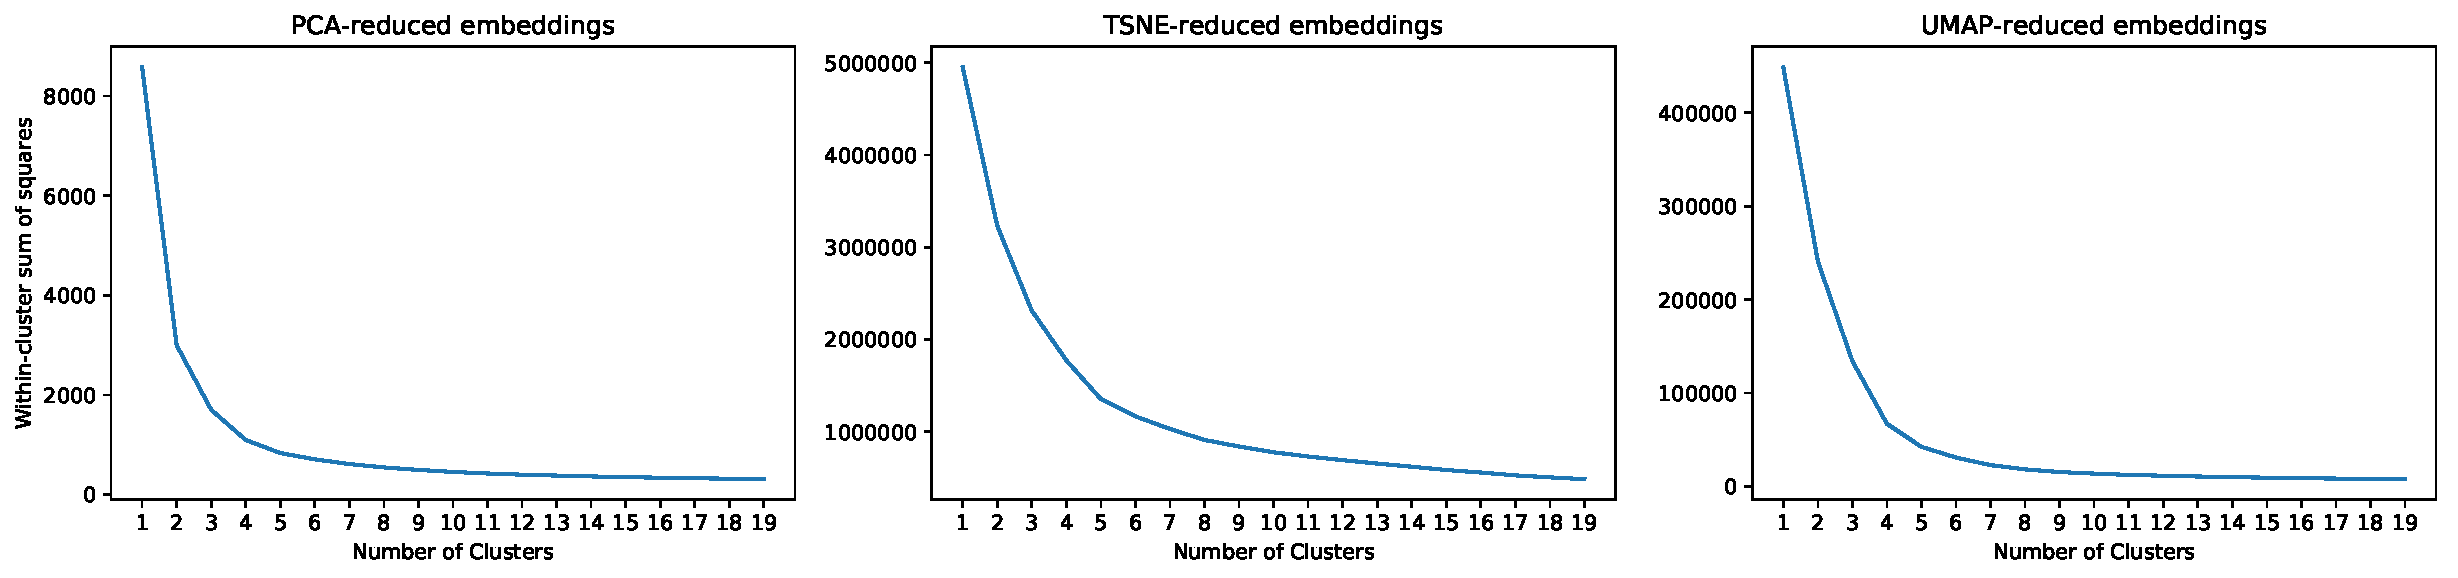
\includegraphics[width=1.0\textwidth]{images/evaluations/Fig38.pdf}\\
	\caption{Elbow plots for reduced embeddings sets.}
	\label{fig:Fig38}
\end{figure}
\begin{figure}[!ht]
	\centering
	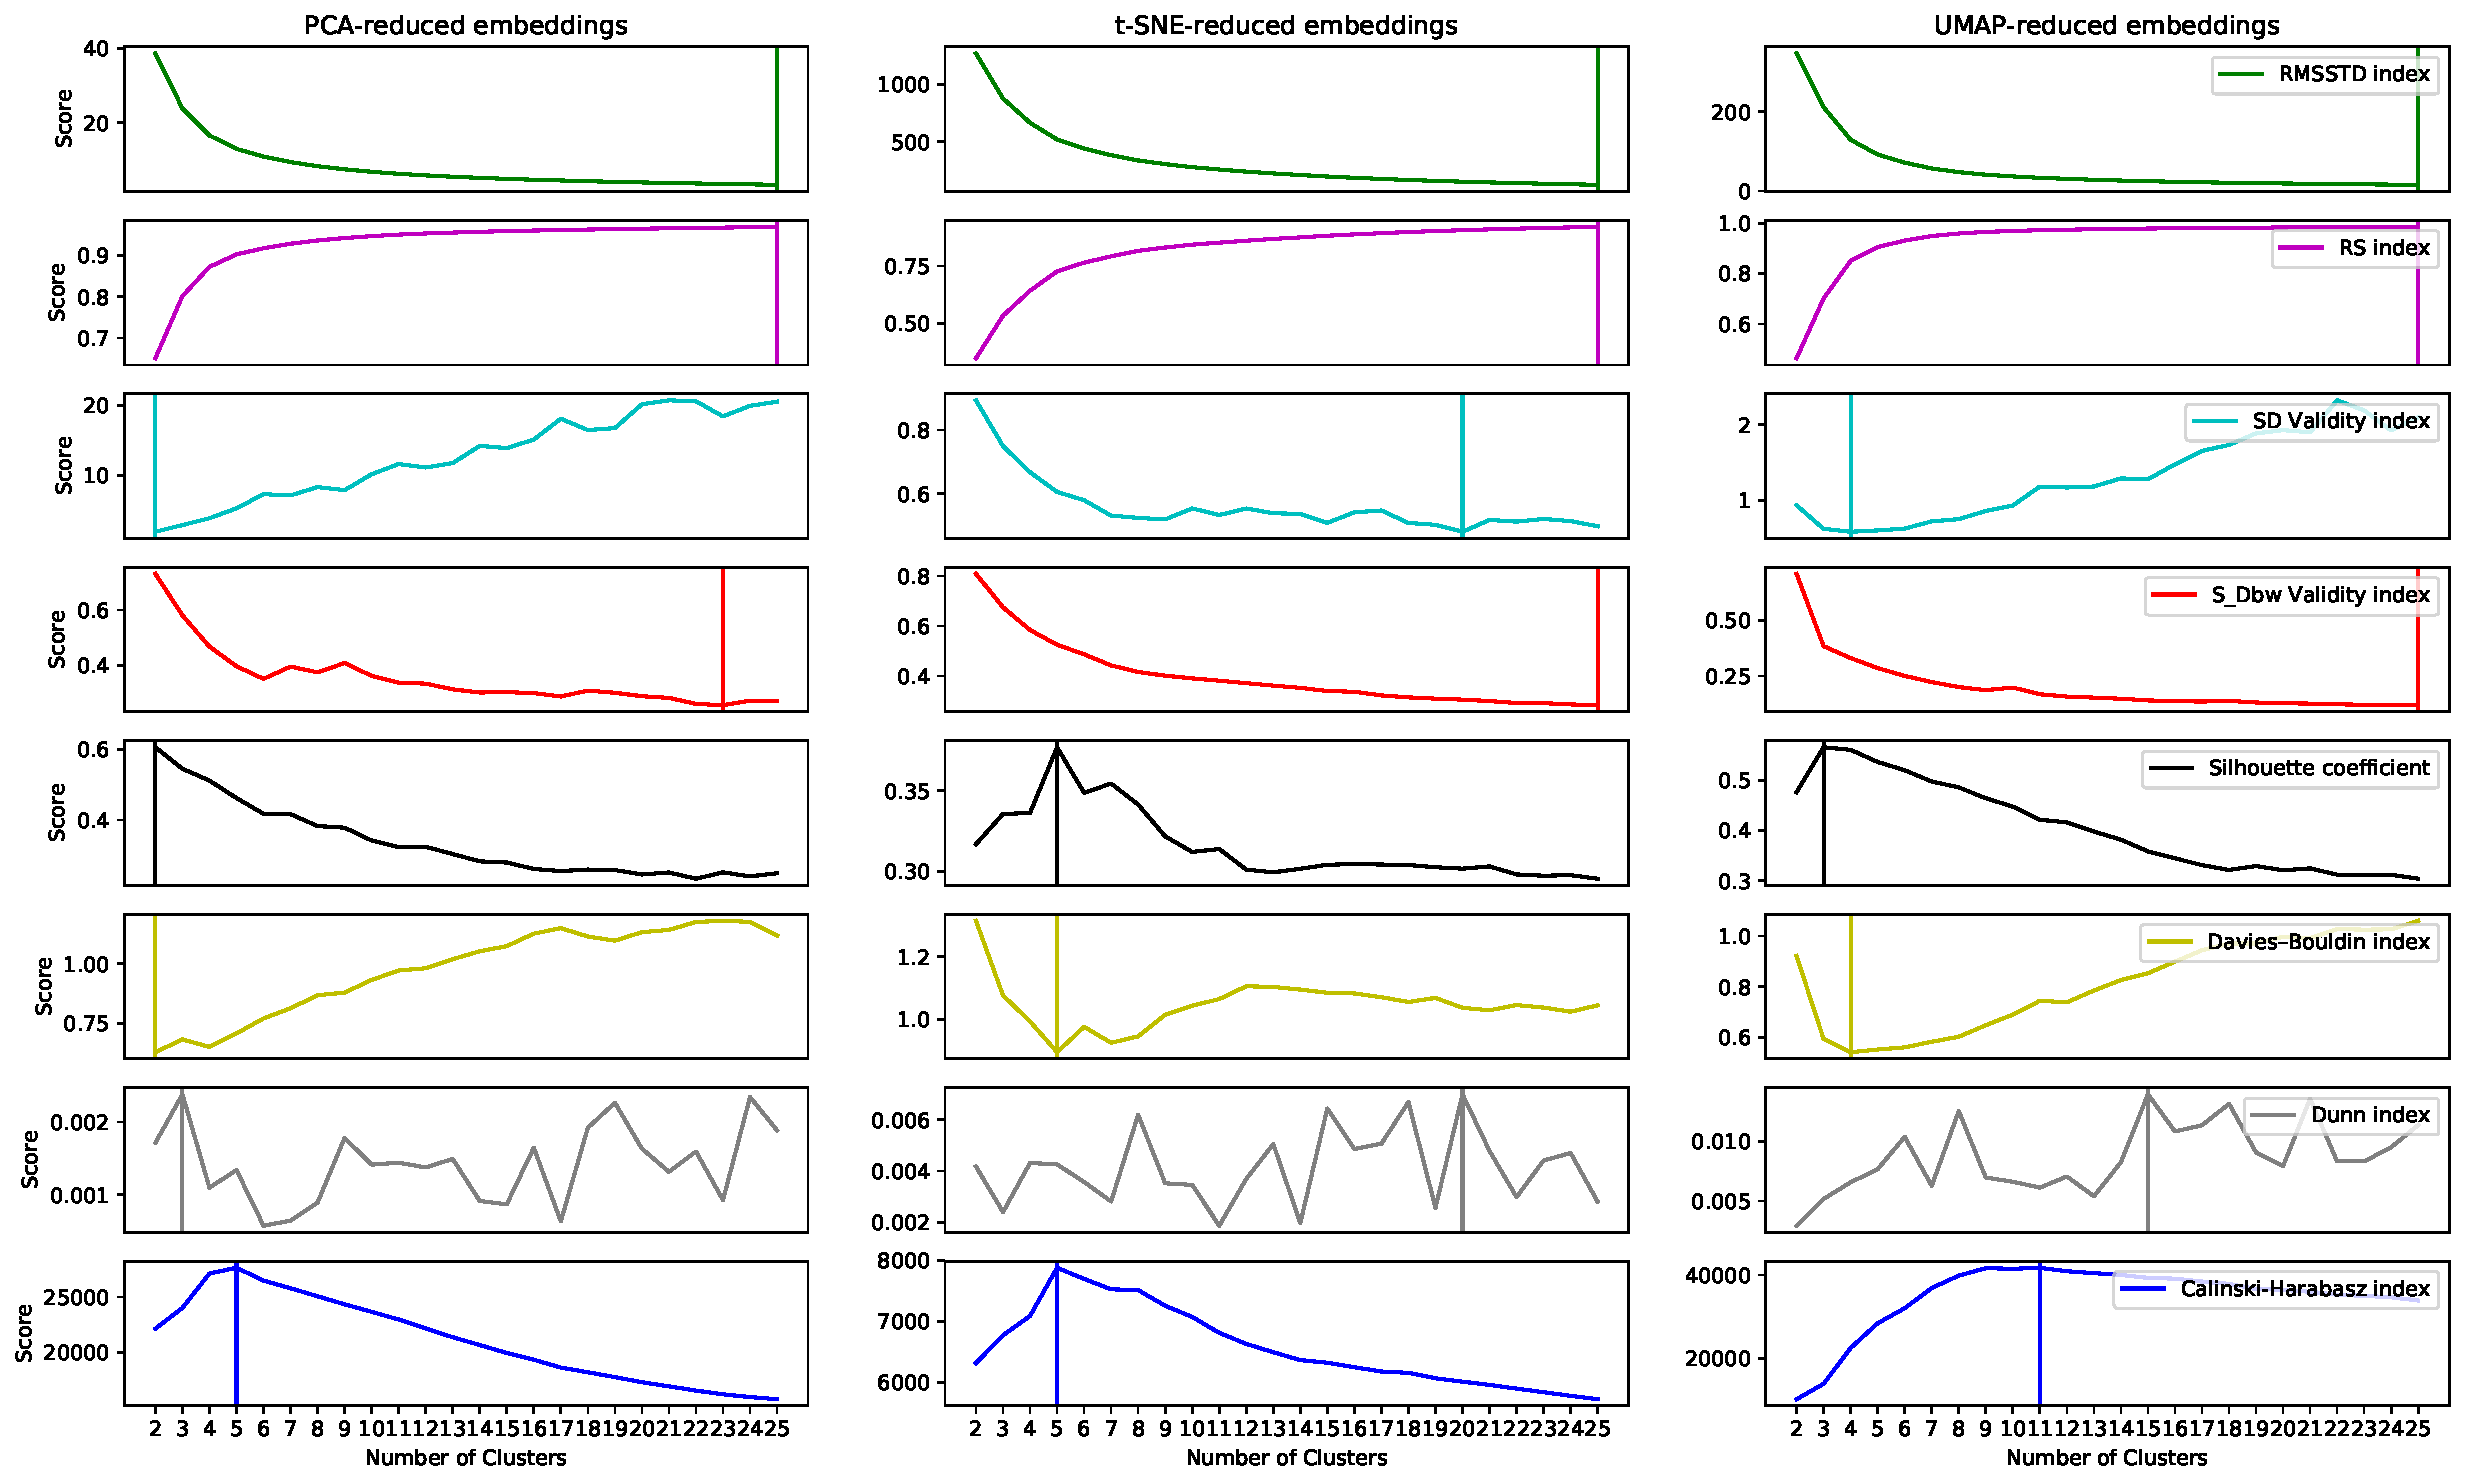
\includegraphics[width=1.0\textwidth]{images/evaluations/Fig39.pdf}\\
	\caption{Evaluation of $k$-means clustering with respect to the number of clusters $k$.}
	\label{fig:Fig39}
\end{figure}
% \fi

Elbow criterion facilitates the choice of an appropriate number of clusters for $k$-means. However, the elbow curves on the~\autoref{fig:Fig38} still leave some room to speculate about the right numbers of clusters: 3 or 4 clusters for PCA embeddings, 5 clusters for t-SNE, and 4 or 5 clusters for UMAP embeddings. To reduce that uncertainty it is helpful to compute the internal clustering measures for different numbers of $k$. ~\autoref{fig:Fig39} provides visualizations of measures' values varying with the increasing numbers of $k$ for every reduced embeddings set. The vertical lines at each plot denote the best choice of $k$ suggested by a particular measure (max or min).

The comprehensive analysis of the metrics from~\autoref{fig:Fig38} and ~\autoref{fig:Fig39} concludes the optimal $k$ equal to 4 for PCA-reduced embeddings, 5 for t-SNE-reduced embeddings, and 4 for UMAP-reduced embeddings. The intuition under this selection is exampled below for the t-SNE-reduced embeddings case:
\begin{enumerate}
    \item on the~\autoref{fig:Fig38} the marginal gain in within-cluster sum of squares drops significantly after the $k = 5$;
    \item on the~\autoref{fig:Fig39} RMSSTD, RS, and S\_Dbw Validity indices are generally higher if the number of clusters grows since they mostly aim at minimizing within-cluster inertia. They are not very meaningful in this case, unlike Silhouette coefficient, Davies–Bouldin, and Calinski-Harabasz indices, that suggest picking $k = 5$;
    \item although Dunn and SD Validity indices do not reach extremum at $k = 5$, they demonstrate slight convex and concave respectively at this point.
\end{enumerate}
The above intuition works for the rest cases for choosing $k$ in $k$-means clustering. ~\autoref{fig:Fig40} shows the resulting $k$-means clustering of initial sets from ~\autoref{fig:Fig37}. Refer to appendix 1-2 for the rest of the cases.  §
% \iffalse
\begin{figure}[!ht]
	\centering
	\includegraphics[width=1.0\textwidth]{images/evaluations/Fig40.pdf}\\
	\caption{Embeddings sets coloured by k-means clusters.}
	\label{fig:Fig40}
\end{figure}
% \fi
\subsubsection{Finding the best $k$-means clustering}
\label{Finding the best $k$-means clustering}
The previous section explains the choice of $k$ in $k$-means clustering. The current section compares clustering results among pipeline's branches ending by $k$-means.~\autoref{tab:tab5} collected the internal clustering metrics values rounded to the third digit (or other where appropriate) for each of nine $k$-means clusterings. The metrics were extensively discussed in the~\ref{Cluster evaluation strategies} along with their respective optima. The closest to optima values of measures are highlighted bold. The best values belong to $k$-means clustering of embeddings learned from the local and global structural components of the network and then reduced by UMAP. This clustering reaches the best or the second-best values in seven metrics out of eight. The visualization of the leading $k$-means clustering in a metric space is depicted on the~\autoref{fig:Fig40} right.

\begin{table}
\begin{center}
\small
\begin{tabular}{lrrrrrrrrrr}
\hline
\multicolumn{1}{l}{ } & \multicolumn{3}{c}{\textbf{loc + time}} & \multicolumn{3}{c}{\textbf{loc + glob}} & \multicolumn{3}{c}{\textbf{loc + time + glob}} \\
\cline{1-1} \cline{2-4} \cline{5-7} \cline{8-10} 
measure & PCA & t-SNE & UMAP & PCA & t-SNE & UMAP & PCA & t-SNE & UMAP & opt\\
\hline
RMSSTD & 44.14 & 791.7 & 158.4 & \textbf{16.53} & 520.4 & 129.5 & 33.60 & 602.8 & 89.72 & min \\
RS     & 0.530 & 0.569 & 0.658 & \textbf{0.873}  & 0.726   & 0.850  & 0.616 & 0.665 & 0.775 & max \\
SD     & 1.998 & 0.725 & 0.857 & 3.864  & 0.605   & \textbf{0.586}  & 2.814 & 0.666 & 1.003 & min \\
S\_Dbw & 0.962 & 0.657 & 0.592 & 0.467  & 0.525   & \textbf{0.330}  & 0.956 & 0.573 & 0.480 & min \\
SC     & 0.506 & 0.350 & 0.431 & 0.511  & 0.377   & \textbf{0.561}  & 0.465 & 0.354 & 0.371 & max \\
DB     & 0.988 & 1.006 & 0.847 & 0.651  & 0.897   & \textbf{0.541}  & 0.946 & 0.917 & 0.879 & min \\
D      & 0.0024 & 0.0025 & \textbf{0.006829} & 0.001  & 0.002 & 0.006567 & 0.0012 & 0.0054 & 0.0055 & max \\
CH     & 6969.6 & 7850.2 & 1449.4 & \textbf{27102.9} & 7880.5 & 22499.8 & 6352.8 & 7862.3 & 10184.8 & max \\
\hline
\end{tabular}
\caption {$k$-means clustering evaluation of the pipeline brunches ended in $k$-means}
\label{tab:tab5}
\end{center}
\end {table}

\subsection{HDBSCAN clustering}

The current section repeats the intuition from the above for determining an appropriate number of clusters and finding the best branch's result for HDBSCAN clustering. For the sake of consistency, the same branches' results will be examined, and evaluations of the rest branches' results are presented in the appendices 1-2.

\subsubsection{Determining the number of clusters}
Unlike $k$-means clustering where a number of clusters is a user-defined parameter, HDBSCAN clustering determines it automatically. However, HDBSCAN requires the set of input hyperparameters: \textit{minimum cluster size, minimum number of samples, alpha} (explained in~\ref{Result evaluation}). The best combination will be found automatically via a grid search algorithm. The three hyperparameters are varying between the certain appropriate ranges suggested by HDBSCAN creators in~\cite{mcinnes2017hdbscan}. HDBSCAN clustering is validated on 27 combinations of three hyperparameters by the set of six internal clustering measures (the initial eight measures from~\ref{Concept evaluation} except two working only for globular clusters - RMSSTD and RS indices). Similar to the $k$-means clustering evaluation, the best HDBSCAN clustering result is defined by the best measures magnitudes.

~\autoref{fig:Fig41} shows the varying values of the internal clustering metrics over different combinations of HDBSCAN hyperparameters for the embeddings learned from the local and global structural components of the network. In case of t-SNE-reduced embeddings set, the best choice of three hyperparameters are 20 for minimum cluster size, 5 for minimum number of samples, and 0.25 for alpha.~\autoref{fig:Fig42} visualizes the reduced embeddings from ~\autoref{fig:Fig37} coloured according to the HDBSCAN defined clusters (in this case 2 clusters in every set). Refer to the appendix 1-2 for HDBSCAN clustering evaluations of the other branches' results ending by HDBSCAN.

% \iffalse
\begin{figure}[!ht]
	\centering
	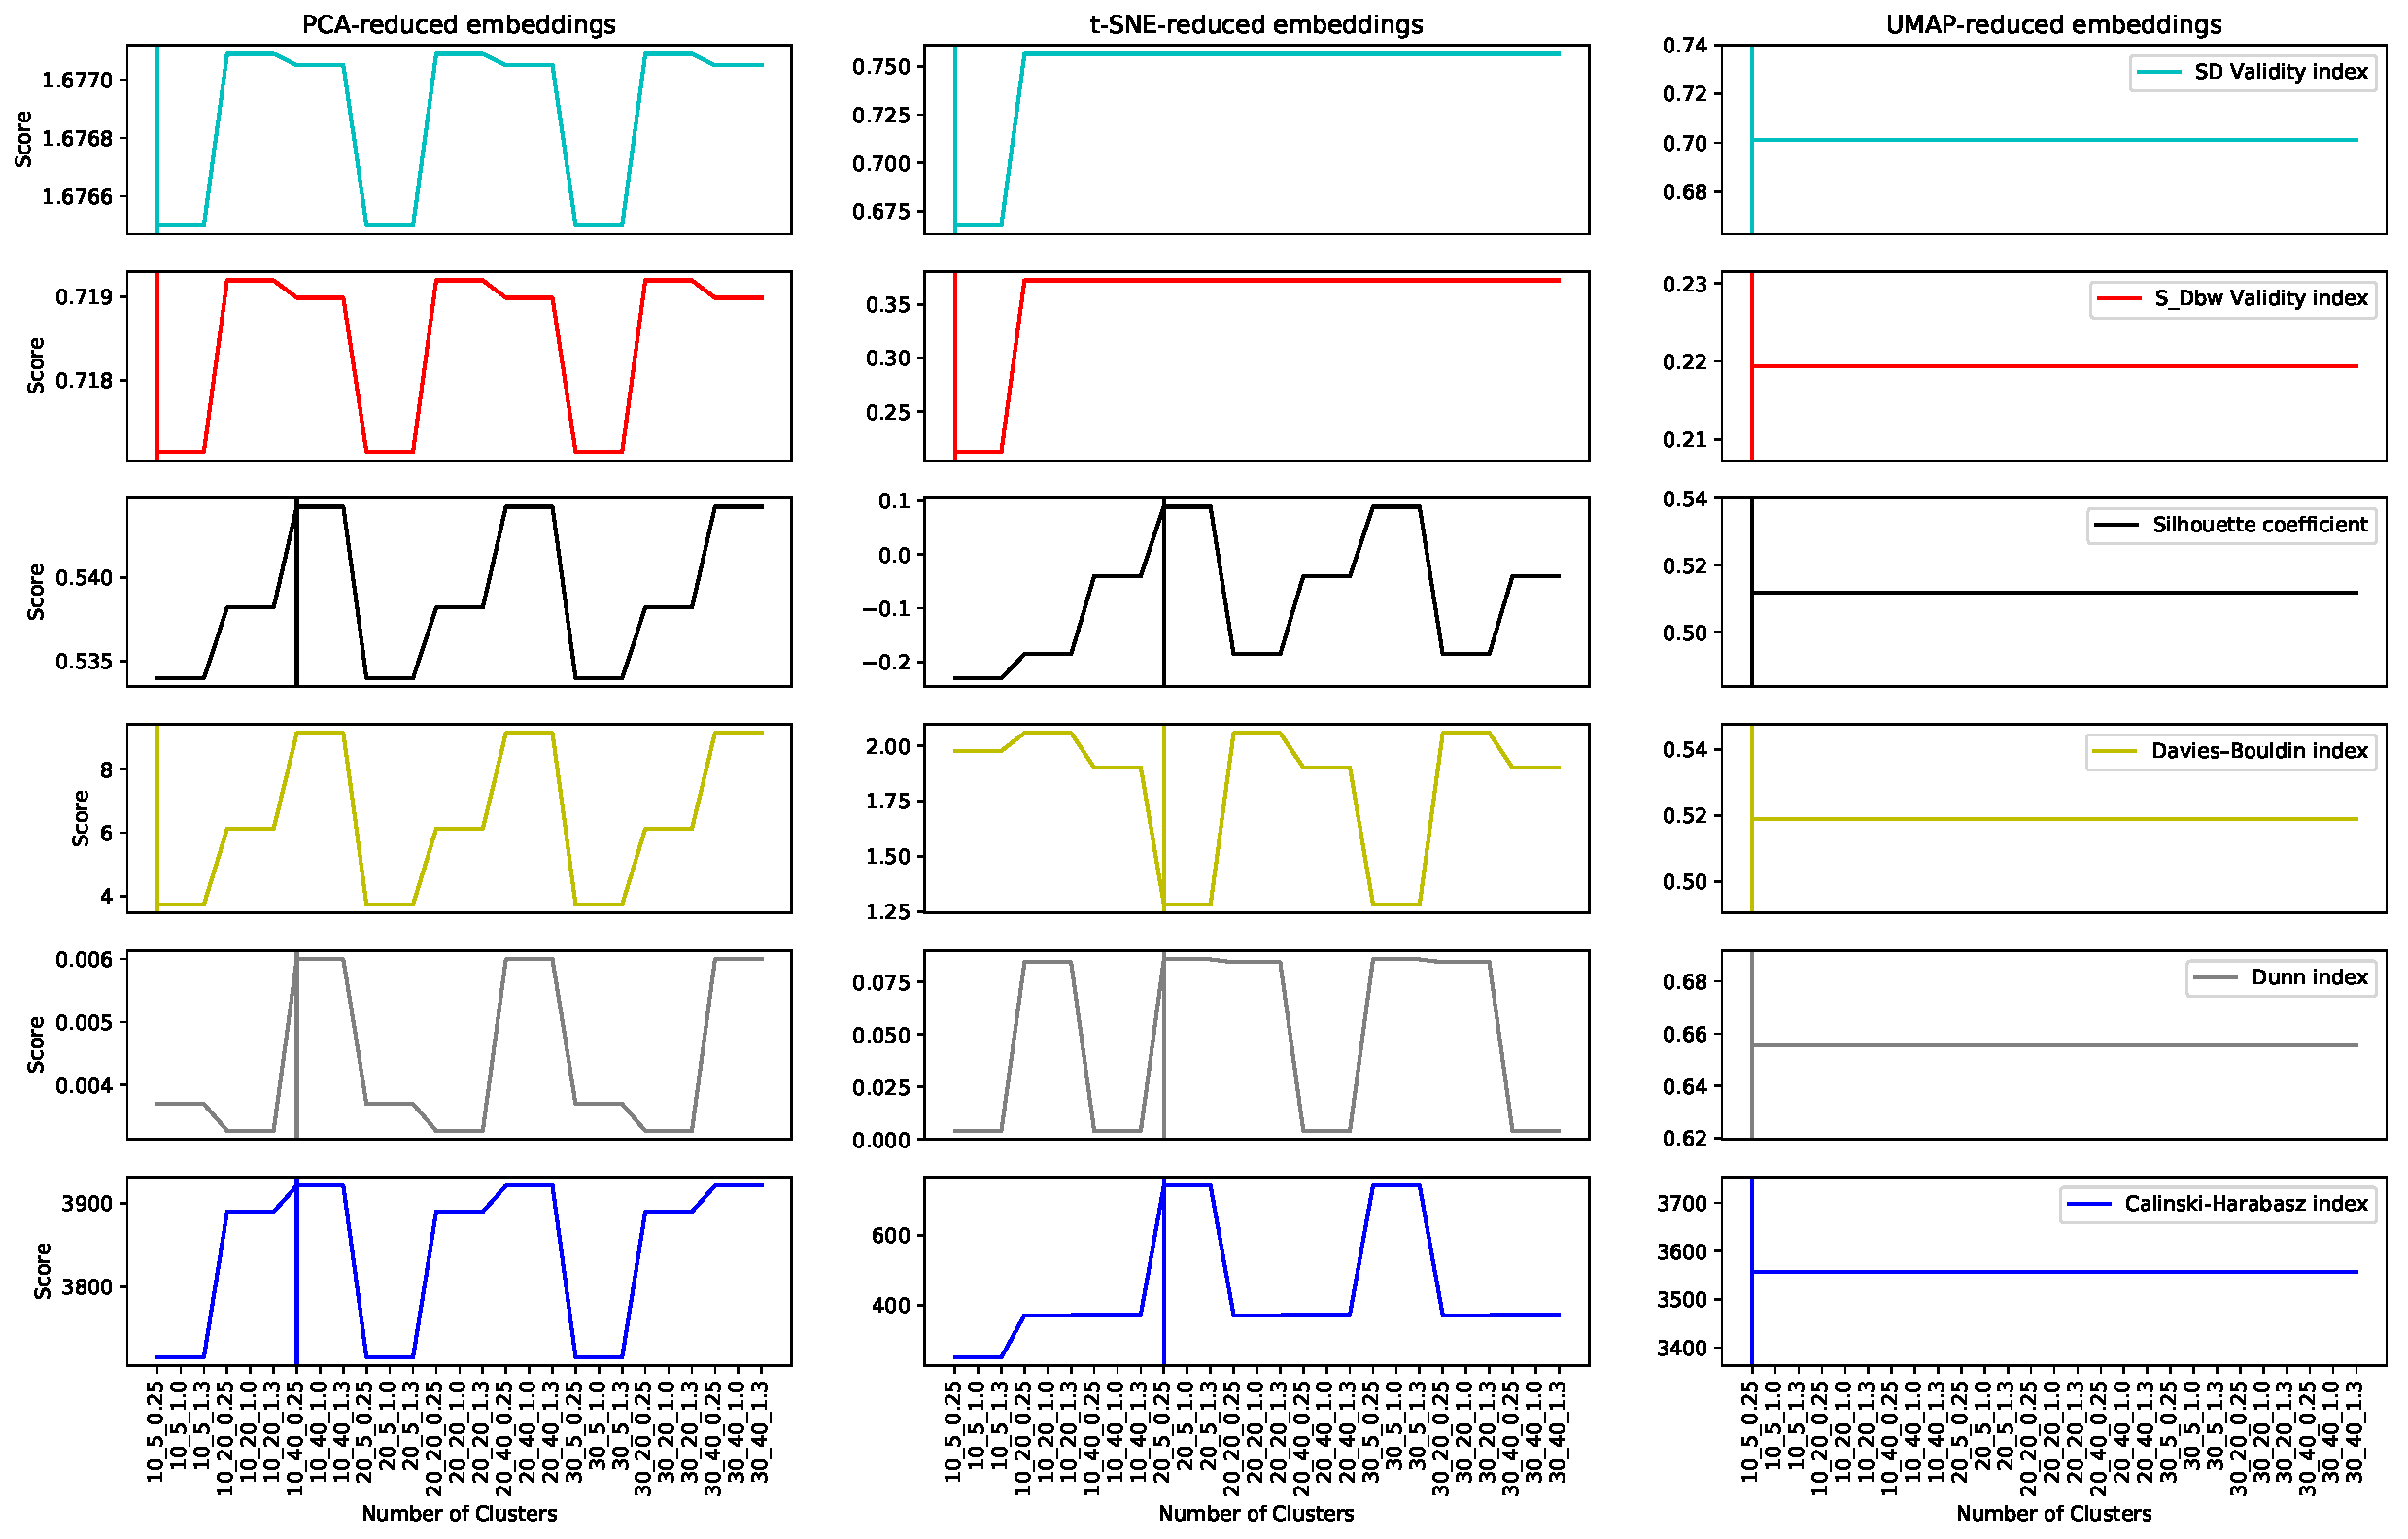
\includegraphics[width=1.0\textwidth]{images/evaluations/Fig41.pdf}\\
	\caption{Evaluation of HDBSCAN clustering with respect to the combination of hyperparameters (x axis: minimum cluster size\_minimum number of samples\_alpha).}
	\label{fig:Fig41}
\end{figure}
\begin{figure}[!ht]
	\centering
	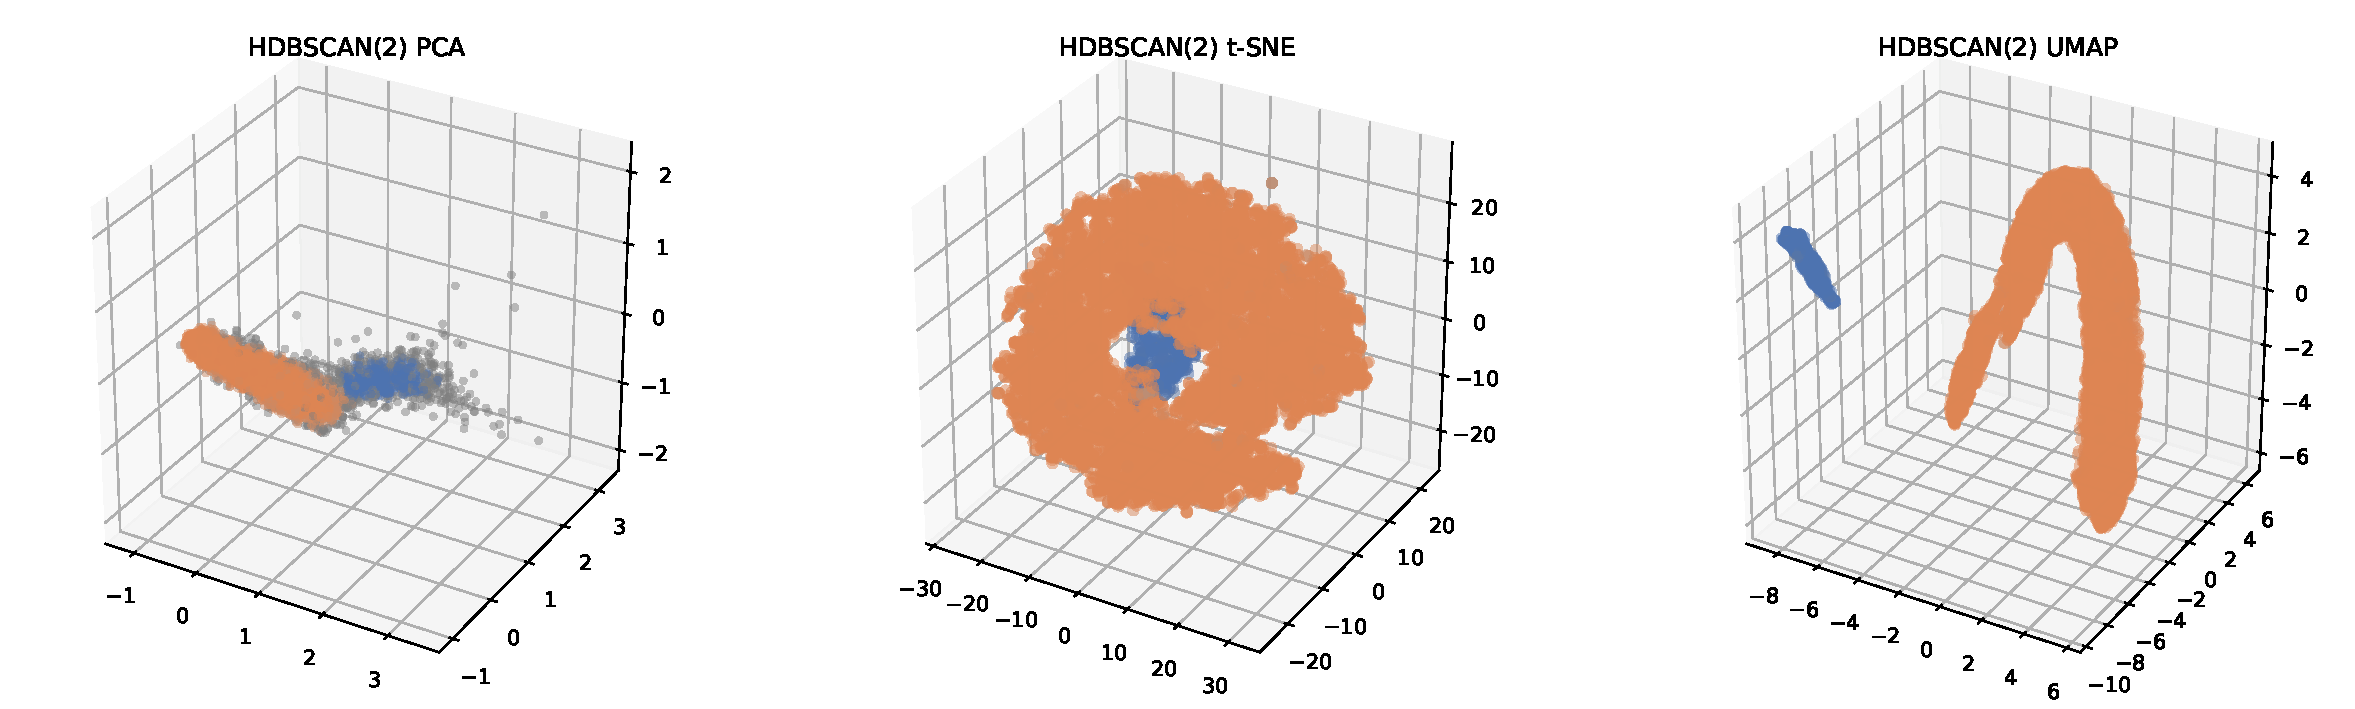
\includegraphics[width=1.0\textwidth]{images/evaluations/Fig42.pdf}\\
	\caption{Embeddings sets coloured by HDBSCAN clusters.}
	\label{fig:Fig42}
\end{figure}
% \fi

\subsubsection{Finding the best HDBSCAN clustering}
The best HDBSCAN clustering will be chosen from the nine possible reduced data sets.~\autoref{tab:tab6} presents the internal clustering metrics' values for HDBSCAN clustering. The best clustering is determined likewise~\ref{Finding the best $k$-means clustering}. In the current case, UMAP-reduced data set learned from the local and global structural components of the network is superior over others. It has the best values for two metrics (highlighted bold) and the second-best values for another two.

\begin{table}
\begin{center}
\small
\begin{tabular}{lrrrrrrrrrr}
\hline
\multicolumn{1}{l}{ } & \multicolumn{3}{c}{\textbf{loc + time}} & \multicolumn{3}{c}{\textbf{loc + glob}} & \multicolumn{3}{c}{\textbf{loc + time + glob}} \\
\cline{1-1} \cline{2-4} \cline{5-7} \cline{8-10} 
measure & PCA & t-SNE & UMAP & PCA & t-SNE & UMAP & PCA & t-SNE & UMAP & opt\\
\hline
SD     & 1.681 & 0.674 & 0.856 & 1.677 & 0.757 & 0.701 & 1.902 & \textbf{0.571} & 2.737 & min \\
S\_Dbw & 0.931 & 0.204 & \textbf{0.068} & 0.717 & 0.372 & 0.219 & 1.167 & 0.317 & 0.214 & min \\
SC     & 0.508 & 0.010 & -0.077 & \textbf{0.533} & 0.089 & 0.512 & 0.464 & -0.376 & -0.193 & max \\
DB     & 1.682 & 0.861 & 3.590 & 3.740 & 1.283 & \textbf{0.519} & 1.676 & 1.405 & 1.155 & min \\
D      & 0.0039 & 0.0127 & 0.0011 & 0.0037 & 0.086 & \textbf{0.656} & 0.0031 & 0.0014 & 0.0013&max\\
CH     & 838.4 & 117.9 & 128.2 & \textbf{3715.2} & 742.1 & 3557.9 & 850.4 & 313.6 & 477.8 & max \\
\hline
\end{tabular}
\caption {HDBSCAN clustering evaluation of the pipeline brunches ended in HDBSCAN}
\label{tab:tab6}
\end{center}
\end {table}

\subsection{Comparison clustering results of $k$-means and HDBSCAN}
\label{Comparison clustering results of $k$-means and HDBSCAN}

After identification of the optimal values for hyperparameters, exploring and comparing the clustering results of differently reduced datasets, the last step is to find the best clustering result of the pipeline.~\autoref{fig:Fig42} visualizes the two leading clustering splits and ~\autoref{tab:tab7} compares them by means of the internal clustering measures. The precise comparison of measures' magnitudes does not define a clear winner in this case. Furthermore, the three metrics out of six (Silhouette coefficient, S\_Dbw Validity and Davies–Bouldin indices) have very close values for two results. The remainder of the chapter is devoted to interpretation and comparison of these results. Additionally, the detailed evaluations of other clustering results that have not been mentioned above can be found in appendices 1-2.
% \iffalse
\begin{figure}[!ht]
	\centering
	\includegraphics[width=1.0\textwidth]{images/evaluations/Fig43.pdf}\\
	\caption{From left to right: Embeddings learned from the local and global structural components of the network; the same coloured by k-means clusters' labels (k=4); the same coloured by HDBSCAN clusters' labels (2 clusters).}
	\label{fig:Fig43}
\end{figure}
% \fi

\begin{table}
\begin{center}
\small
\begin{tabular}{lrrrrrrrrrr}
\hline
measure & loc+glob->UMAP->k-means(4) & loc+glob->UMAP->HDBSCAN(2) & opt\\
\hline
SD      & \textbf{0.586} & 0.701 & min \\
S\_Dbw  & 0.330 & \textbf{0.219} & min \\
SC      & \textbf{0.561} & 0.512 & max \\
DB      & 0.541 & \textbf{0.519} & min \\
D       & 0.006567 & \textbf{0.656} & max\\
CH      & \textbf{22499.8} & 3557.9 & max \\
\hline
\end{tabular}
\caption {Comparison of the two best clustering results from all branches of the pipeline.}
\label{tab:tab7}
\end{center}
\end {table}

\section{Interpretation of clustering results}
This section takes a close look at the resulting clusters from~\ref{Comparison clustering results of $k$-means and HDBSCAN}. K-means clustering analysis generates 4 clusters from UMAP-reduced dataset learned from local and global structural components of the financial network. As the global structural component is represented by nodes' degree in the network, it is worth to look at the degree distribution of the nodes grouped by clusters on~\autoref{fig:Fig44}. As it can be seen, four clusters have very different degree distribution of nodes: 
    \begin{itemize}
        \item The first cluster consists of 4 103 nodes and their overall degree varies around 4,7. Its standard deviation from the mean is comparatively low - 3,9 (violet data points on the centre plot on the~\autoref{fig:Fig43}).
        \item The second cluster contains 3 840 nodes with mean of degrees - 17,9 and standard deviation - 8,7 (yellow data points on the centre plot of the~\autoref{fig:Fig43}).
        \item The third cluster counts 3 181 nodes. Mean of degrees - 47,5 and standard deviation - 8,7 (blue data points on the centre plot on the~\autoref{fig:Fig43}).
        \item The forth cluster contains 754 nodes with mean of degrees equal to 165.9 and standard deviation - 118.8 (green data points on the centre plot on the~\autoref{fig:Fig43})
    \end{itemize}
    
% \iffalse
\begin{figure}[!ht]
	\centering
	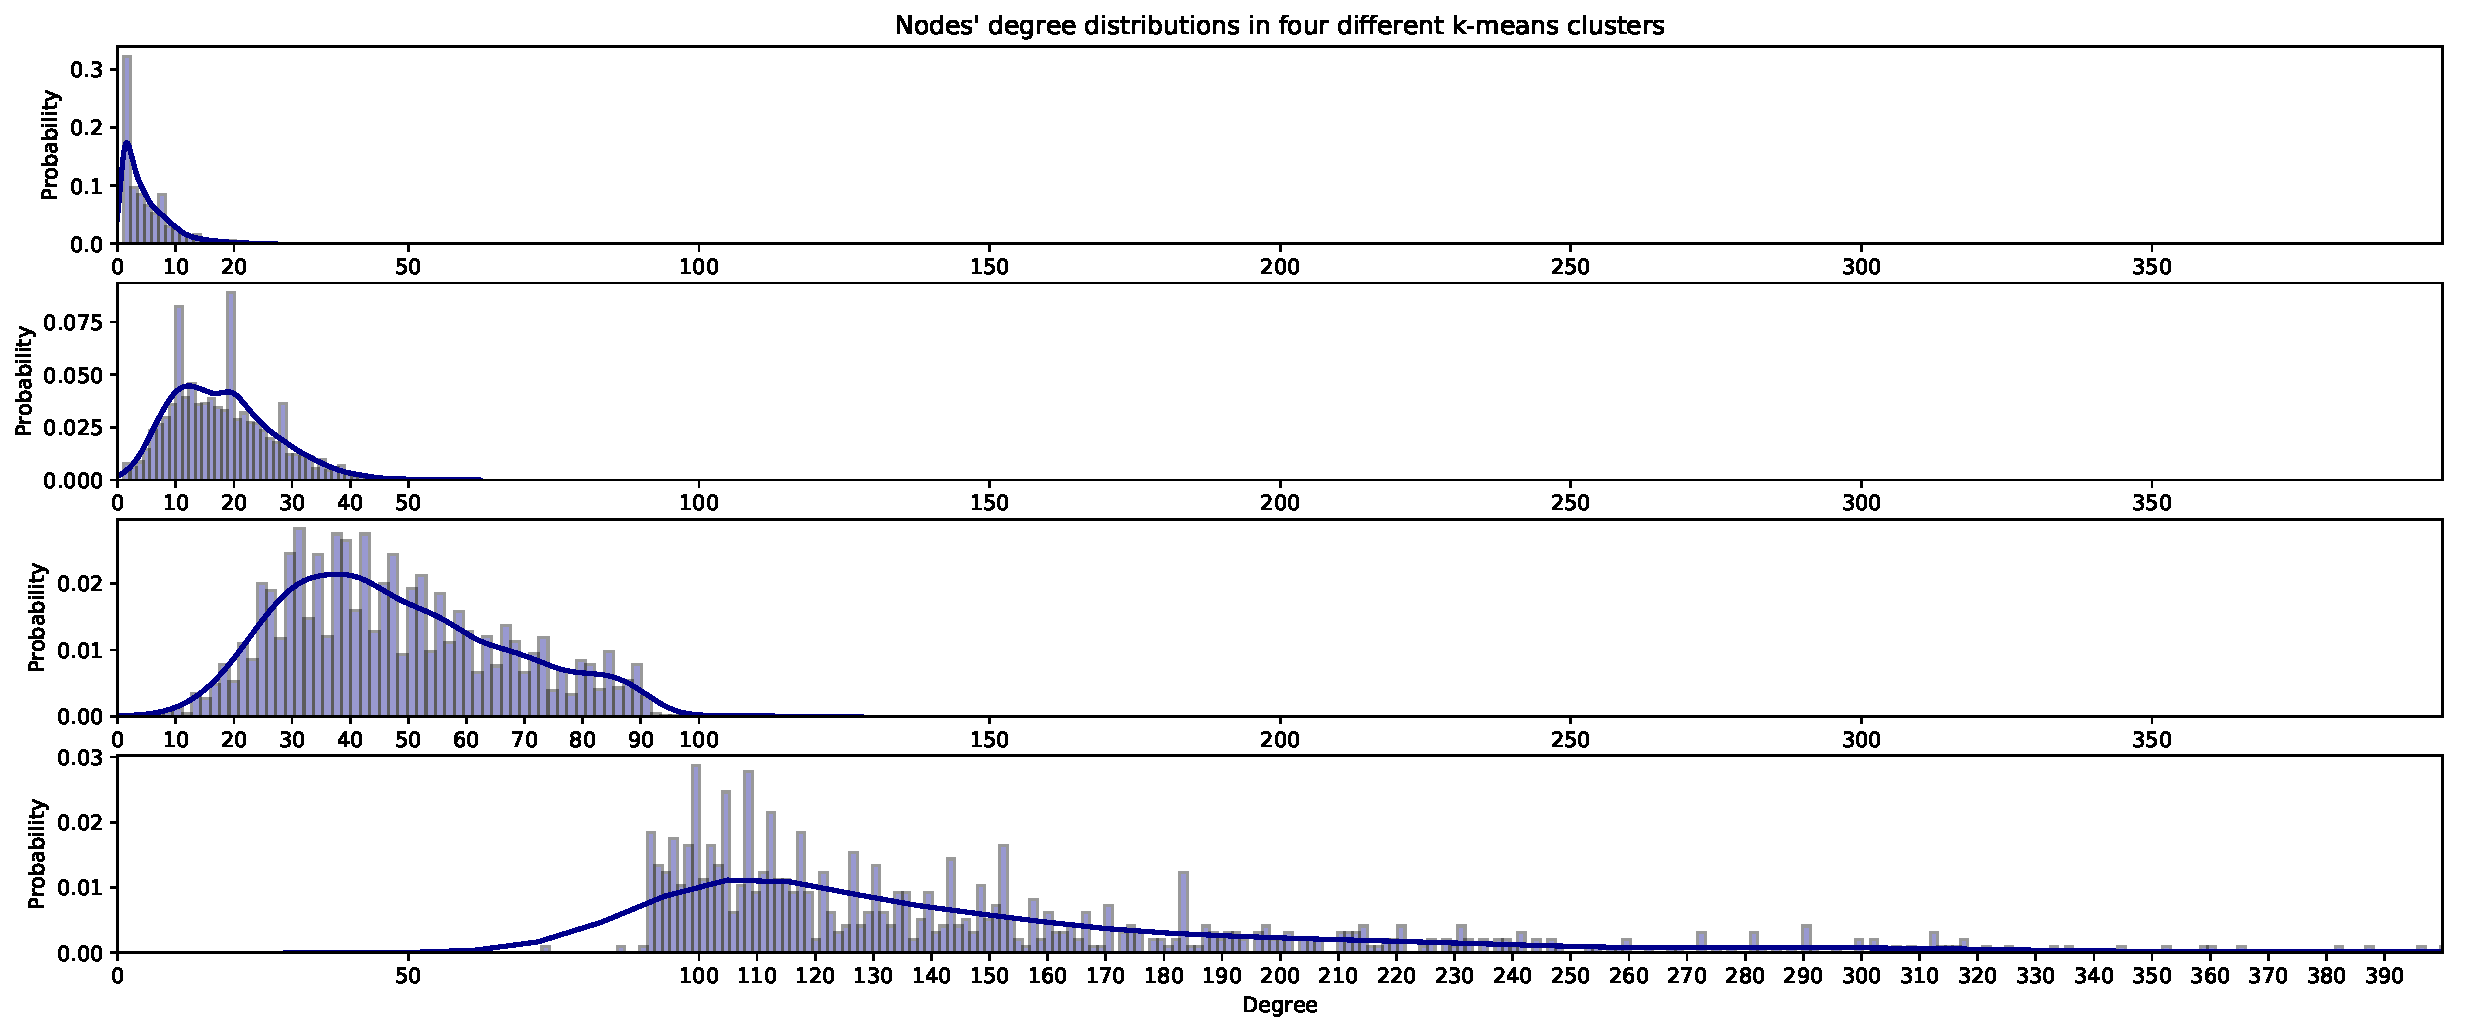
\includegraphics[width=1.0\textwidth]{images/evaluations/Fig44.pdf}\\
	\caption{Degree distribution of nodes in 4 k-means defined clusters. From the first to the fourth cluster top to bottom}
	\label{fig:Fig44}
\end{figure}

The first cluster is the most numerous since more than a third of the network's nodes have a small degree: ~36,2\% of nodes have degree lower than 10. However, this cluster is quite compact and adjoins with another cluster by one side. The reason for this lies in the local component affected the embeddings. The smooth transition from the first cluster to the second means that low-degree nodes usually communicate with the nodes of the second cluster, which have slightly higher degrees. The second cluster transits smoothly to the third. This observation highlights the network structure where nodes generally with small degrees tend to connect to nodes with slightly higher degrees and so on. In general, low-degree nodes are not directly connected to the network's hubs of the highest degrees. 

The fourth cluster of green colour on the~\autoref{fig:Fig43} consists of the nodes characterized by the highest degrees. This cluster is compact and well-separated from the rest of the network's nodes because of the particular degree classes allocation strategy. 12 degree classes were initially distinguished in the network. Nodes of the degrees from 1 to 90 were distributed over the first 11 classes while the rest nodes of the highest degrees from 90 to 1364 were assigned to the last class. The ordered sequences include hubs of different high degrees surrounded by the same degree class. This leads to the skip-gram model producing embeddings for hubs closer together because of the same degree class and pays less attention to the local component. That is why the low-dimensional representation places the cluster of hubs aside from other clusters. To confirm this reasoning, a more gradual degree classes split of 16 classes was tested on the~\autoref{fig:Fig46}. The smooth transition between clusters is clearly tracked here.

% \iffalse
\begin{figure}[!ht]
	\centering
	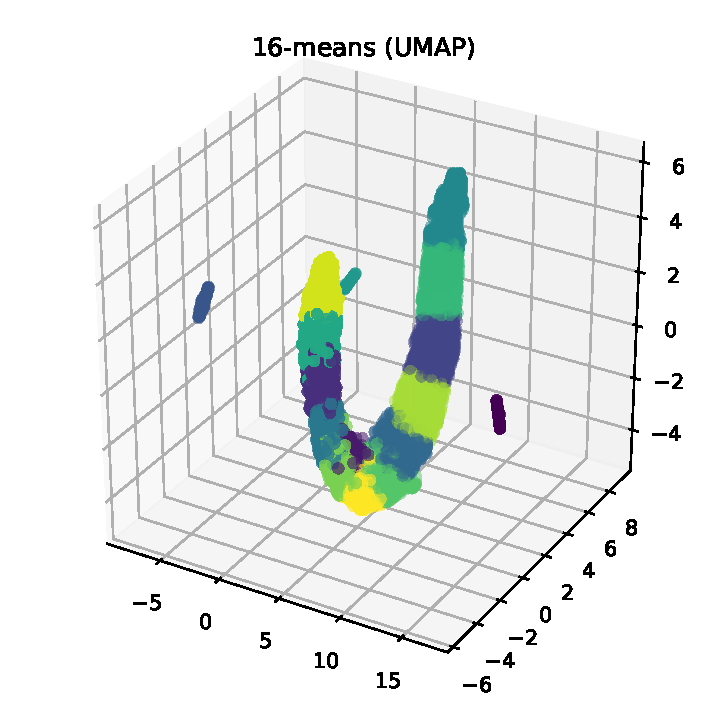
\includegraphics[width=0.4\textwidth]{images/evaluations/Fig46.pdf}\\
	\caption{Pipeline branch outcome visualization: local+global components -> UMAP -> $k$-means clustering (k=16).}
	\label{fig:Fig46}
\end{figure}
% \fi

The HDBSCAN outputs more coarse clusters than $k$-means under the all combinations of hyperparameters. The 27 combinations of hyperparameters min\_cluster\_size $\in$ [10,20,30], min\_samples $\in$ [5,20,40], and alpha $\in$ [0.25, 1.0, 1.3] leads to the same result of two separated clusters on the~\autoref{fig:Fig43} right. The nodes' degree distribution by clusters is on the~\autoref{fig:Fig44}. 
\begin{figure}[H]
	\centering
	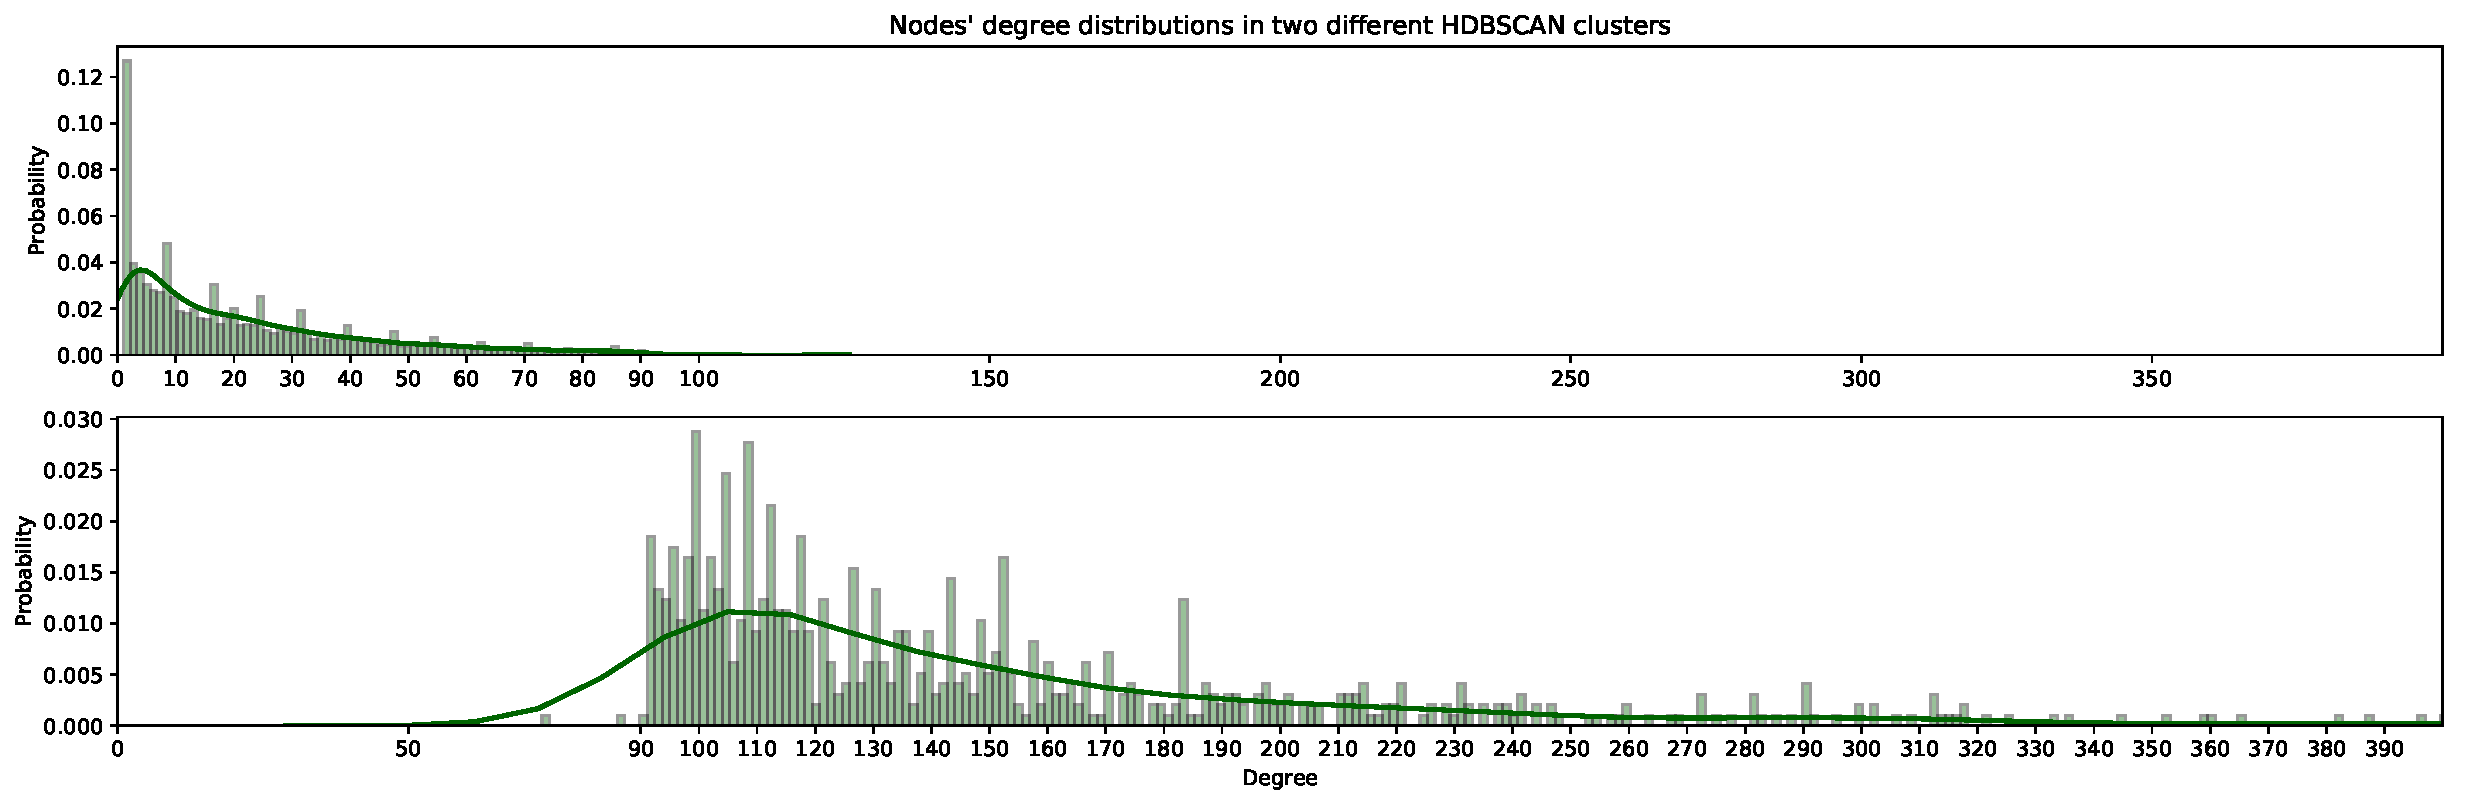
\includegraphics[width=1.0\textwidth]{images/evaluations/Fig45.pdf}\\
	\caption{Degree distribution of nodes in 2 HDBSCAN defined clusters. From the first to the second cluster top to bottom}
	\label{fig:Fig45}
\end{figure}
% \fi
    \begin{itemize}
        \item The first cluster consists of 11 126 nodes with the mean degree equal to 21.5. Its standard deviation is lower than the second cluster has - 20.9 (yellow data points on the right plot on the~\autoref{fig:Fig43}).
        \item the second cluster of HDBSCAN repeats the fourth cluster in $k$-means clustering: 754 nodes, mean of degrees equal to 165.9, standard deviation - 118.8 (violet data points on the right plot on the~\autoref{fig:Fig43})
    \end{itemize}
HDBSCAN finds dense non-globular clusters. The fact that the first cluster is relatively numerous evidences that nodes with degrees lower than 90 are well connected in the underlying network. Furthermore, these UMAP-reduced embeddings in the 3d metric space are dense enough to assign them to the same cluster. The rest separately allocated nodes serve as hubs in the network and belong to the second cluster.

The obtained experiment's result above demonstrated the analytical ability of UMAP approach to derive critical, meaningful information from the high-dimensional data better than others. The $k$-means clustering can capture the finer clusters due to the manual tuning of the hyperparameter $k$, whereas HDBSCAN relies mostly on the density of the points in a space and finds coarse-grained clusters unless clusters are separated with troughs of low density. Visualizations of the original financial network with nodes colored by $k$-means and HDBSCAN clustering labels can be found in the appendix 3.

\section{Summary}
This chapter presented the evaluation of the clustering results as the overall pipeline evaluation. The experiments on the real-world financial data set demonstrated the superiority of particular pipeline's branches over others for the particular input data set. The evaluation have been done by the set of internal clustering measures.

The result of the data science pipeline is strongly affected by the input data set and chosen hyperparameters. Therefore, this chapter suggested the ensemble of indices and heuristics for hyperparameters tuning as well as described the practical example of processing the real-world data set.

The chapter presented and compared the results from two pipeline's branches with the best outcomes according to the set of measures. The analysis of the other branches' results can be found in the appendices 1-2.

The next and last chapter of the current thesis will briefly revise the main points discussed in the work, summarize the main findings, provide some critical reviews, and point the direction for the future improvements.